\section*{Aufgabe 1}
\subsection*{1a) und b)}
In dieser Aufgabe war das Ising-Modell zu untersuchen für verschiedene Gittergrößen
und Dimensionen sowie verschiedene β-Werte. Dazu soll die mittlere Magnetisierung 
und Energie berechnet werden sowie eine grobe Fehlerabschätzung durchgeführt werden.
Der entsprechende Code ist in \lref{main} dargestellt.

\lstinputlisting[label=lst:main,caption={main.cpp}]{../code/main.cpp}

Der entsprechende Output ist in \lref{output} dargestellt, wobei jeweils alle
zehn Block-Ergebnisse und der resultierende Mittelwert gezeigt wird.

\begin{lstlisting}[caption=Output von \lref{main},label=lst:output,language=]
>make run11 # Parameter: L=4 D=1 beta=0.5
./main 4  1 0 0.2 0.5 0
magnetization: 0.26200
energy: -0.60780
magnetization: 0.25375
energy: -0.60605
magnetization: 0.22875
energy: -0.59815
magnetization: 0.23950
energy: -0.59980
magnetization: 0.24520
energy: -0.60474
magnetization: 0.22905
energy: -0.60071
magnetization: 0.24650
energy: -0.60400
magnetization: 0.23440
energy: -0.60258
magnetization: 0.24615
energy: -0.59953
magnetization: 0.25395
energy: -0.59979
magnetization mean: 0.24393 +- 0.01048
energy mean: -0.60231 +- 0.00305

>make run12 # Parameter: L=20 D=1 beta=0.5
./main 20 1 0 0.2 0.5 0
magnetization: 0.26463
energy: -0.54155
magnetization: 0.27494
energy: -0.54729
magnetization: 0.27165
energy: -0.54149
magnetization: 0.26015
energy: -0.53921
magnetization: 0.26923
energy: -0.54255
magnetization: 0.26515
energy: -0.53777
magnetization: 0.26571
energy: -0.54076
magnetization: 0.26452
energy: -0.54312
magnetization: 0.26755
energy: -0.54179
magnetization: 0.26374
energy: -0.54183
magnetization mean: 0.26673 +- 0.00404
energy mean: -0.54174 +- 0.00238

>make run13 # Parameter: L=4 D=2 beta=0.4
./main 4  2 0 0.2 0.4 0
magnetization: 0.65239
energy: -1.62093
magnetization: 0.67997
energy: -1.62055
magnetization: 0.65949
energy: -1.61342
magnetization: 0.65594
energy: -1.62176
magnetization: 0.66391
energy: -1.62038
magnetization: 0.60964
energy: -1.62240
magnetization: 0.63048
energy: -1.61397
magnetization: 0.67096
energy: -1.63464
magnetization: 0.64725
energy: -1.61415
magnetization: 0.64846
energy: -1.61989
magnetization mean: 0.65185 +- 0.01910
energy mean: -1.62021 +- 0.00581

>make run14 # Parameter: L=10 D=2 beta=0.4
./main 10 2 0 0.2 0.4 0
magnetization: 0.80770
energy: -1.64835
magnetization: 0.80956
energy: -1.65612
magnetization: 0.81115
energy: -1.65741
magnetization: 0.81976
energy: -1.67137
magnetization: 0.81493
energy: -1.66166
magnetization: 0.81479
energy: -1.66611
magnetization: 0.81675
energy: -1.66751
magnetization: 0.81089
energy: -1.65845
magnetization: 0.81640
energy: -1.66833
magnetization: 0.81428
energy: -1.66257
magnetization mean: 0.81362 +- 0.00352
energy mean: -1.66179 +- 0.00655
\end{lstlisting}

Wie man erkennen kann, stimmen die \texttt{mean}-Werte gut mit den Referenzwerten
überein.

\subsection*{1c)}
Hier wird eine Hysteresekurve für die mittlere Magnetisierung und für die mittlere
Energie untersucht. Der Code ist bereits in \lref{main} dargestellt, die resultierenden
Plots sind in \fref{ev1} bis \fref{mv2} dargestellt.

\begin{figure}
  \centering
  \subfloat[Mittlere Energie für  Setup 1]{\label{fig:ev1}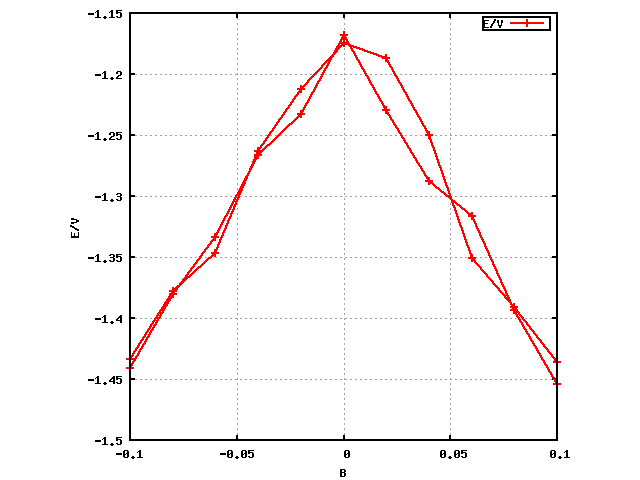
\includegraphics[width=0.5\textwidth]{../tmp/ev_1}}
  \subfloat[Mittlere Magnetisierung für Setup 1]{\label{fig:mv1}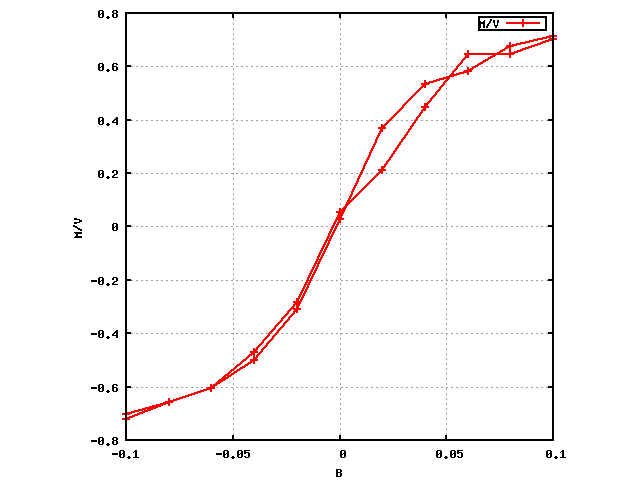
\includegraphics[width=0.5\textwidth]{../tmp/mv_1}}  \\
  \subfloat[Mittlere Energie für Setup 2]{\label{fig:ev2}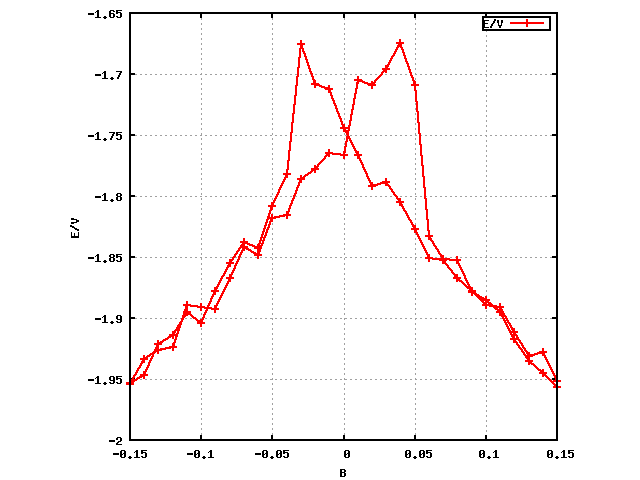
\includegraphics[width=0.5\textwidth]{../tmp/ev_2}}
  \subfloat[Mittlere Magnetisierung für Setup 2]{\label{fig:m2}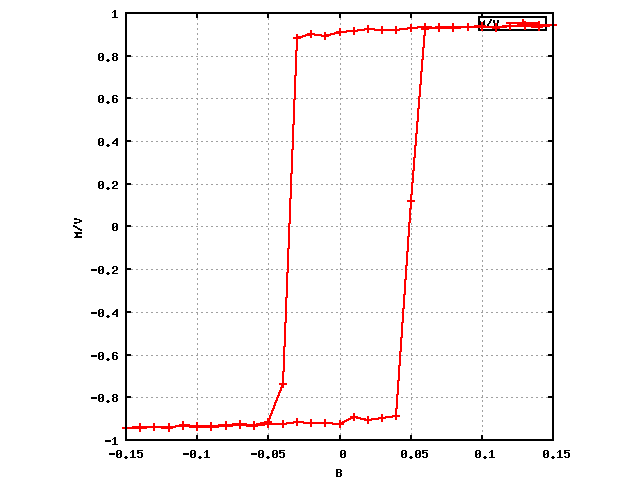
\includegraphics[width=0.5\textwidth]{../tmp/mv_2}}
  \caption{Plot-Ergebnisse}
  \label{fig:plots}
\end{figure}

% Hier Text

